
%% bare_conf.tex
%% V1.4b
%% 2015/08/26
%% by Michael Shell
%% See:
%% http://www.michaelshell.org/
%% for current contact information.
%%
%% This is a skeleton file demonstrating the use of IEEEtran.cls
%% (requires IEEEtran.cls version 1.8b or later) with an IEEE
%% conference paper.
%%
%% Support sites:
%% http://www.michaelshell.org/tex/ieeetran/
%% http://www.ctan.org/pkg/ieeetran
%% and
%% http://www.ieee.org/

%%*************************************************************************
%% Legal Notice:
%% This code is offered as-is without any warranty either expressed or
%% implied; without even the implied warranty of MERCHANTABILITY or
%% FITNESS FOR A PARTICULAR PURPOSE! 
%% User assumes all risk.
%% In no event shall the IEEE or any contributor to this code be liable for
%% any damages or losses, including, but not limited to, incidental,
%% consequential, or any other damages, resulting from the use or misuse
%% of any information contained here.
%%
%% All comments are the opinions of their respective authors and are not
%% necessarily endorsed by the IEEE.
%%
%% This work is distributed under the LaTeX Project Public License (LPPL)
%% ( http://www.latex-project.org/ ) version 1.3, and may be freely used,
%% distributed and modified. A copy of the LPPL, version 1.3, is included
%% in the base LaTeX documentation of all distributions of LaTeX released
%% 2003/12/01 or later.
%% Retain all contribution notices and credits.
%% ** Modified files should be clearly indicated as such, including  **
%% ** renaming them and changing author support contact information. **
%%*************************************************************************


% *** Authors should verify (and, if needed, correct) their LaTeX system  ***
% *** with the testflow diagnostic prior to trusting their LaTeX platform ***
% *** with production work. The IEEE's font choices and paper sizes can   ***
% *** trigger bugs that do not appear when using other class files.       ***                          ***
% The testflow support page is at:
% http://www.michaelshell.org/tex/testflow/

\documentclass[conference]{IEEEtran}
% Some Computer Society conferences also require the compsoc mode option,
% but others use the standard conference format.
%
% If IEEEtran.cls has not been installed into the LaTeX system files,
% manually specify the path to it like:
% \documentclass[conference]{../sty/IEEEtran}





% Some very useful LaTeX packages include:
% (uncomment the ones you want to load)



\usepackage{fancyhdr}

% *** MISC UTILITY PACKAGES ***
%
%\usepackage{ifpdf}
% Heiko Oberdiek's ifpdf.sty is very useful if you need conditional
% compilation based on whether the output is pdf or dvi.
% usage:
% \ifpdf
%   % pdf code
% \else
%   % dvi code
% \fi
% The latest version of ifpdf.sty can be obtained from:
% http://www.ctan.org/pkg/ifpdf
% Also, note that IEEEtran.cls V1.7 and later provides a builtin
% \ifCLASSINFOpdf conditional that works the same way.
% When switching from latex to pdflatex and vice-versa, the compiler may
% have to be run twice to clear warning/error messages.






% *** CITATION PACKAGES ***
%
%\usepackage{cite}
% cite.sty was written by Donald Arseneau
% V1.6 and later of IEEEtran pre-defines the format of the cite.sty package
% \cite{} output to follow that of the IEEE. Loading the cite package will
% result in citation numbers being automatically sorted and properly
% "compressed/ranged". e.g., [1], [9], [2], [7], [5], [6] without using
% cite.sty will become [1], [2], [5]--[7], [9] using cite.sty. cite.sty's
% \cite will automatically add leading space, if needed. Use cite.sty's
% noadjust option (cite.sty V3.8 and later) if you want to turn this off
% such as if a citation ever needs to be enclosed in parenthesis.
% cite.sty is already installed on most LaTeX systems. Be sure and use
% version 5.0 (2009-03-20) and later if using hyperref.sty.
% The latest version can be obtained at:
% http://www.ctan.org/pkg/cite
% The documentation is contained in the cite.sty file itself.






% *** GRAPHICS RELATED PACKAGES ***
%
\ifCLASSINFOpdf
  % \usepackage[pdftex]{graphicx}
  % declare the path(s) where your graphic files are
  % \graphicspath{{../pdf/}{../jpeg/}}
  % and their extensions so you won't have to specify these with
  % every instance of \includegraphics
  % \DeclareGraphicsExtensions{.pdf,.jpeg,.png}
\else
  % or other class option (dvipsone, dvipdf, if not using dvips). graphicx
  % will default to the driver specified in the system graphics.cfg if no
  % driver is specified.
  % \usepackage[dvips]{graphicx}
  % declare the path(s) where your graphic files are
  % \graphicspath{{../eps/}}
  % and their extensions so you won't have to specify these with
  % every instance of \includegraphics
  % \DeclareGraphicsExtensions{.eps}
\fi
% graphicx was written by David Carlisle and Sebastian Rahtz. It is
% required if you want graphics, photos, etc. graphicx.sty is already
% installed on most LaTeX systems. The latest version and documentation
% can be obtained at: 
% http://www.ctan.org/pkg/graphicx
% Another good source of documentation is "Using Imported Graphics in
% LaTeX2e" by Keith Reckdahl which can be found at:
% http://www.ctan.org/pkg/epslatex
%
% latex, and pdflatex in dvi mode, support graphics in encapsulated
% postscript (.eps) format. pdflatex in pdf mode supports graphics
% in .pdf, .jpeg, .png and .mps (metapost) formats. Users should ensure
% that all non-photo figures use a vector format (.eps, .pdf, .mps) and
% not a bitmapped formats (.jpeg, .png). The IEEE frowns on bitmapped formats
% which can result in "jaggedy"/blurry rendering of lines and letters as
% well as large increases in file sizes.
%
% You can find documentation about the pdfTeX application at:
% http://www.tug.org/applications/pdftex





% *** MATH PACKAGES ***
%
%\usepackage{amsmath}
% A popular package from the American Mathematical Society that provides
% many useful and powerful commands for dealing with mathematics.
%
% Note that the amsmath package sets \interdisplaylinepenalty to 10000
% thus preventing page breaks from occurring within multiline equations. Use:
%\interdisplaylinepenalty=2500
% after loading amsmath to restore such page breaks as IEEEtran.cls normally
% does. amsmath.sty is already installed on most LaTeX systems. The latest
% version and documentation can be obtained at:
% http://www.ctan.org/pkg/amsmath





% *** SPECIALIZED LIST PACKAGES ***
%
%\usepackage{algorithmic}
% algorithmic.sty was written by Peter Williams and Rogerio Brito.
% This package provides an algorithmic environment fo describing algorithms.
% You can use the algorithmic environment in-text or within a figure
% environment to provide for a floating algorithm. Do NOT use the algorithm
% floating environment provided by algorithm.sty (by the same authors) or
% algorithm2e.sty (by Christophe Fiorio) as the IEEE does not use dedicated
% algorithm float types and packages that provide these will not provide
% correct IEEE style captions. The latest version and documentation of
% algorithmic.sty can be obtained at:
% http://www.ctan.org/pkg/algorithms
% Also of interest may be the (relatively newer and more customizable)
% algorithmicx.sty package by Szasz Janos:
% http://www.ctan.org/pkg/algorithmicx




% *** ALIGNMENT PACKAGES ***
%
%\usepackage{array}
% Frank Mittelbach's and David Carlisle's array.sty patches and improves
% the standard LaTeX2e array and tabular environments to provide better
% appearance and additional user controls. As the default LaTeX2e table
% generation code is lacking to the point of almost being broken with
% respect to the quality of the end results, all users are strongly
% advised to use an enhanced (at the very least that provided by array.sty)
% set of table tools. array.sty is already installed on most systems. The
% latest version and documentation can be obtained at:
% http://www.ctan.org/pkg/array


% IEEEtran contains the IEEEeqnarray family of commands that can be used to
% generate multiline equations as well as matrices, tables, etc., of high
% quality.




% *** SUBFIGURE PACKAGES ***
%\ifCLASSOPTIONcompsoc
%  \usepackage[caption=false,font=normalsize,labelfont=sf,textfont=sf]{subfig}
%\else
%  \usepackage[caption=false,font=footnotesize]{subfig}
%\fi
% subfig.sty, written by Steven Douglas Cochran, is the modern replacement
% for subfigure.sty, the latter of which is no longer maintained and is
% incompatible with some LaTeX packages including fixltx2e. However,
% subfig.sty requires and automatically loads Axel Sommerfeldt's caption.sty
% which will override IEEEtran.cls' handling of captions and this will result
% in non-IEEE style figure/table captions. To prevent this problem, be sure
% and invoke subfig.sty's "caption=false" package option (available since
% subfig.sty version 1.3, 2005/06/28) as this is will preserve IEEEtran.cls
% handling of captions.
% Note that the Computer Society format requires a larger sans serif font
% than the serif footnote size font used in traditional IEEE formatting
% and thus the need to invoke different subfig.sty package options depending
% on whether compsoc mode has been enabled.
%
% The latest version and documentation of subfig.sty can be obtained at:
% http://www.ctan.org/pkg/subfig




% *** FLOAT PACKAGES ***
%
%\usepackage{fixltx2e}
% fixltx2e, the successor to the earlier fix2col.sty, was written by
% Frank Mittelbach and David Carlisle. This package corrects a few problems
% in the LaTeX2e kernel, the most notable of which is that in current
% LaTeX2e releases, the ordering of single and double column floats is not
% guaranteed to be preserved. Thus, an unpatched LaTeX2e can allow a
% single column figure to be placed prior to an earlier double column
% figure.
% Be aware that LaTeX2e kernels dated 2015 and later have fixltx2e.sty's
% corrections already built into the system in which case a warning will
% be issued if an attempt is made to load fixltx2e.sty as it is no longer
% needed.
% The latest version and documentation can be found at:
% http://www.ctan.org/pkg/fixltx2e


%\usepackage{stfloats}
% stfloats.sty was written by Sigitas Tolusis. This package gives LaTeX2e
% the ability to do double column floats at the bottom of the page as well
% as the top. (e.g., "\begin{figure*}[!b]" is not normally possible in
% LaTeX2e). It also provides a command:
%\fnbelowfloat
% to enable the placement of footnotes below bottom floats (the standard
% LaTeX2e kernel puts them above bottom floats). This is an invasive package
% which rewrites many portions of the LaTeX2e float routines. It may not work
% with other packages that modify the LaTeX2e float routines. The latest
% version and documentation can be obtained at:
% http://www.ctan.org/pkg/stfloats
% Do not use the stfloats baselinefloat ability as the IEEE does not allow
% \baselineskip to stretch. Authors submitting work to the IEEE should note
% that the IEEE rarely uses double column equations and that authors should try
% to avoid such use. Do not be tempted to use the cuted.sty or midfloat.sty
% packages (also by Sigitas Tolusis) as the IEEE does not format its papers in
% such ways.
% Do not attempt to use stfloats with fixltx2e as they are incompatible.
% Instead, use Morten Hogholm'a dblfloatfix which combines the features
% of both fixltx2e and stfloats:
%
% \usepackage{dblfloatfix}
% The latest version can be found at:
% http://www.ctan.org/pkg/dblfloatfix




% *** PDF, URL AND HYPERLINK PACKAGES ***
%
%\usepackage{url}
% url.sty was written by Donald Arseneau. It provides better support for
% handling and breaking URLs. url.sty is already installed on most LaTeX
% systems. The latest version and documentation can be obtained at:
% http://www.ctan.org/pkg/url
% Basically, \url{my_url_here}.




% *** Do not adjust lengths that control margins, column widths, etc. ***
% *** Do not use packages that alter fonts (such as pslatex).         ***
% There should be no need to do such things with IEEEtran.cls V1.6 and later.
% (Unless specifically asked to do so by the journal or conference you plan
% to submit to, of course. )



\usepackage[onelanguage,linesnumbered,ruled,inoutnumbered]{algorithm2e}


\usepackage{graphicx}


% correct bad hyphenation here
\hyphenation{op-tical net-works semi-conduc-tor}


\usepackage{syntax}
\grammarindent 80pt

\usepackage{newfloat}
% declare the floating environment {Grammar}
% this will also define \listofGrammars:
\DeclareFloatingEnvironment[
% the file extension for the file used to create the list:
fileext   = logr,% don't use log here!
% the heading for the list:
listname  = {List of Grammars},
% the name used in captions:
name      = Grammar,
% the default floating parameters if the environment is used
% without optional argument:
placement = htp
]{Grammar}




\begin{document}
%
% paper title
% Titles are generally capitalized except for words such as a, an, and, as,
% at, but, by, for, in, nor, of, on, or, the, to and up, which are usually
% not capitalized unless they are the first or last word of the title.
% Linebreaks \\ can be used within to get better formatting as desired.
% Do not put math or special symbols in the title.
\title{Automated Design of Hyper-Heuristics Components to Solve the PSP Problem with HP Model}


% author names and affiliations
% use a multiple column layout for up to three different
% affiliations

\author{\IEEEauthorblockN{Vidal D. Fontoura}
\IEEEauthorblockA{Federal University of Parana \\ (DInf-UFPR), Curitiba - PR, Brazil\\
Email: vdfontoura@inf.ufpr.br}
\and
\IEEEauthorblockN{Aurora T. R. Pozo}
\IEEEauthorblockA{Federal University of Parana \\ (DInf-UFPR), Curitiba - PR, Brazil\\
Email: aurora@inf.ufpr.br}
\and
\IEEEauthorblockN{Roberto Santana}
\IEEEauthorblockA{University of the Basque Country\\
San Sebastian, Spain\\
Email: roberto.santana@ehu.es
}}

% conference papers do not typically use \thanks and this command
% is locked out in conference mode. If really needed, such as for
% the acknowledgment of grants, issue a \IEEEoverridecommandlockouts
% after \documentclass


% for over three affiliations, or if they all won't fit within the width
% of the page, use this alternative format:
% 
%\author{\IEEEauthorblockN{Michael Shell\IEEEauthorrefmark{1},
%Homer Simpson\IEEEauthorrefmark{2},
%James Kirk\IEEEauthorrefmark{3}, 
%Montgomery Scott\IEEEauthorrefmark{3} and
%Eldon Tyrell\IEEEauthorrefmark{4}}
%\IEEEauthorblockA{\IEEEauthorrefmark{1}School of Electrical and Computer Engineering\\
%Georgia Institute of Technology,
%Atlanta, Georgia 30332--0250\\ Email: see http://www.michaelshell.org/contact.html}
%\IEEEauthorblockA{\IEEEauthorrefmark{2}Twentieth Century Fox, Springfield, USA\\
%Email: homer@thesimpsons.com}
%\IEEEauthorblockA{\IEEEauthorrefmark{3}Starfleet Academy, San Francisco, California 96678-2391\\
%Telephone: (800) 555--1212, Fax: (888) 555--1212}
%\IEEEauthorblockA{\IEEEauthorrefmark{4}Tyrell Inc., 123 Replicant Street, Los Angeles, California 90210--4321}}




% use for special paper notices
%\IEEEspecialpapernotice{(Invited Paper)}




% make the title area
\maketitle


    % Copyright information
          \thispagestyle{plain}
          \fancypagestyle{plain}{
            \fancyhf{} % clear all header and footer fields
            \fancyfoot[L]{978-1-5090-4601-0/17/\$31.00~\copyright2017~IEEE} % change here the copyright notice
            \renewcommand{\headrulewidth}{0pt}
            \renewcommand{\footrulewidth}{0pt}
          }
        

% As a general rule, do not put math, special symbols or citations
% in the abstract
\begin{abstract}
	The Protein Structure Prediction (PSP) problem is one of the modern most challenging problems from science. Simplified protein models are usually applied to simulate and study some characteristics of the protein folding process. Hence, many heuristic strategies have been applied in order to find simplified protein structures in which the protein configuration has the minimal energy. However, these strategies have difficulties in finding the optimal solutions to the longer sequences of amino-acids, due to the complexity of the problem and the huge amount of local optima. Hyper heuristics have proved to be useful in this type of context since they try to combine different heuristics strengths into a single framework. However, there is lack of work addressing the automated design of hyper-heuristics components. This paper proposes GEHyPSP, an approach which aims to achieve generation, through grammatical evolution, of selection mechanisms and acceptance criteria for a hyper-heuristic framework applied to PSP problem. We investigate the strengths and weaknesses of our approach on a benchmark of simplified protein models. GEHyPSP was able to reach the best known results for 7 instances from 11 that composed the benchmark set used to evaluate the approach.
	
	
 
%	TODO: Should we mention in the abstract at least one line
% related to the results achieved by this approach
	
%	Sabar et al. \cite{sabar2015automatic} proposed the automated design of high level heuristics to a hyper-heuristic framework and evaluated its performance by applying in the 6 domain problems from HyFlex \cite{ochoa2012hyflex} framework. The work of Sabar et al. \cite{sabar2015automatic} influenced this paper to chase 
%

	

\end{abstract}

% no keywords




% For peer review papers, you can put extra information on the cover
% page as needed:
% \ifCLASSOPTIONpeerreview
% \begin{center} \bfseries EDICS Category: 3-BBND \end{center}
% \fi
%
% For peerreview papers, this IEEEtran command inserts a page break and
% creates the second title. It will be ignored for other modes.
\IEEEpeerreviewmaketitle



\section{Introduction}

%%TODO: Vidal, try to inject some ¨ variation¨  in the definitions you use, for instance, in the definition of proteins and other concepts.
%If you search in google ¨Protein play a fundamental role in nature. These struc-
%tures made of amino acids participate in many important tasks that guarantee the correct functioning of living cells. ¨ you will find the previous protein paper that begins exactly as this paper does.
%Conferences and journals have algorithms that compute the amount of self-plagiarism of a paper by searching on internet for this type of patters.
%
%So, my advice, go paragraph by paragraph in the introduction and don´t be afraid to leave your personal mark by modifying the way things are said. I will later review the paper and if you introduce mistakes we will correct them. 
Proteins execute an essential role in nature, they are responsible of many important functions for the living cells. Proteins can be seen as amino-acids structures  that guarantee the correct operation of many process from the biological entities. These structures are product of the so-called protein folding process where an unfolded chain of amino-acids is transformed into its final/native structure.

%The protein structure prediction (PSP) has a broad range of  medical and biotechnology applications. For instance: synthesis of new proteins and folds \cite{wang2012structural}, structure based synthesis of new drugs \cite{davis2009rosettaligand}, refinement of theoretical models obtained by comparative modeling \cite{qian2004improvement, krieger2009improving}, and
%obtaining experimental structures from incomplete nuclear magnetic resonance data  \cite{shen2009novo}.  

%The task of determining the native structures of proteins is challenging even for the modern super computers. The difficulty raises up due to the huge search space to test all possible conformation that a sequence of amino-acids can adopt. There are many models to represent proteins structures and can be used to simulate the folding process. Extremely detailed models exist however these representations are computationally very expensive. Hence, many authors \cite{custodio2004investigation,hsu2003growth,lin2011protein,unger1993genetic,santana2008component,custodio2014multiple, garza2012locality} have used simplified models to represent the protein structures.

Many authors \cite{hsu2003growth,santana2008component,custodio2014multiple} have used the Hydrophobic-Polar (HP) \cite{lau1989lattice} simplified model to represent the protein structures. This model simplifies the amino-acids into just two types: hydrophobic (H) or polar (P). Two-dimensional (2D) and three-dimensional (3D) grids can be used to represent the conformations that a protein can adopt. Each conformation in the grid has an associated energy. 

% Para isto, é necessário considerar as interações entre os aminoácidos. Uma interação ocorre quando o par de aminoácidos é adjacente no \textit{grid}/cubo e não é adjacente na sequência. No modelo HP existem apenas três: (HP, HH e PP), mas somente interações hidrofóbicas (HH) influenciam no valor de energia referente a uma conformação \cite{unger1993genetic}. A questão que surge é como buscar, dentre as possíveis conformações, aquela cuja a energia seja mínima.

A wide range of heuristics strategies were proposed to search  conformations of minimum energy in the HP model. Among the approaches that have been applied are genetic algorithms \cite{custodio2014multiple}, ant colony optimization \cite{shmygelska2003improved}, estimation distribution algorithms \cite{santana2008component}, and others [9]. Even though there are different strategies already proposed for the PSP, all face difficulties due to the variability of the characteristics of the fitness landscape for different HP instances.  Some heuristics may work well for some instances but fail to produce good results on instances with different characteristics. 
  
   This fact motivates the study here presented. It is in this type of context that hyper-heuristics are usually a good option. In general the hyper-heuristics frameworks propose a strategy to select, from a pool, the heuristic which is more appropriate for a given stage of the search. Also the hyper-heuristics frameworks define a move acceptance criterion, which is responsible to decide on whether to accept or reject solutions generated by the heuristics. These strategies are high level heuristics from a hyper-heuristic framework. 
 
 Usually the high level heuristics are human-designed approaches although two recent and novelty studies \cite{sabar2012grammatical,sabar2015automatic} proposes the automated design of those components. The results obtained on both studies inspired the idea of automating the design of high level heuristics for a hyper-heuristic framework to solve the PSP problem. Since the PSP with the HP-2D model presents a very complex landscape, automating the design of hyper-heuristic framework could save time, money and human effort. Another motivation of the present study is that the hyper-heuristics frameworks have been applied to other domains and achieved good results. Some examples are the bin packing, personnel scheduling, flowshop, TSP, MAXSAT and CVRP problems \cite{sabar2015automatic}.
 

 
 
% The goal is to use a pool of heuristics proposed in the literature managed by a hyper-heuristic strategy \cite{burke2013hyper}. Since different heuristics have different strengths and weaknesses, it makes sense of merging them into one framework and let a high-level strategy to manage the application of them. 
%
% Burke et al. \cite{burke2010classification} recently defined hyper-heuristics as "an automated methodology for selecting or generating heuristics to solve hard computational search problems". Over the years, these methodologies have succeeded while solving a wide range of real world problems.  However, there is not an in-depth investigation of the suitability of this approach to solve the PSP problem.
 
We introduce GEHyPSP: an automated  mechanism for the generation of high level heuristics for a hyper-heuristic framework to solve the PSP problem. The high level heuristic includes two main components:  a selection mechanism and an acceptance criterion. Both components are generated using grammatical evolution (GE) \cite{ryan1998grammatical}, which is a type of genetic programming (GP) \cite{koza1992genetic}. A set of experiments was designed to evaluate the approach using eleven PSP instances. The results are compared with a the best known results and other human-designed hyper-heuristic approach. 



This paper is organized as follows: in the next section we briefly introduce the Protein Structure Prediction problem and a review of the related works is also presented.  Section \ref{sec:background} presents a background of hyper-heuristics, GP and the GE algorithm. Thereafter, in Section \ref{sec:methodology}, the GEHyPSP  is introduced. In Section \ref{sec:experiments}, the experimental benchmark and numerical results of the conducted experiments are presented. Finally, in Section \ref{sec:conclusion}, the conclusions of the research are given, and further work is discussed.


%TODO: if this is necessary
%The propose of this paper is based on a previous work developed by Sabar et al. \cite{sabar2015automatic}, which generates high level heuristics to six domain problems contained in the hyper-heuristic framework HyFlex \cite{ochoa2012hyflex}.

\section{Protein Structure Prediction} \label{sec:proteinfolding}


Proteins are macromolecules composed by an alphabet of twenty different amino-acids, also referred to as residues. An amino-acid is formed by a peptide backbone and a distinctive side chain group. The peptide bond is defined by an amino group and a carboxyl group connected to an alpha carbon to which a hydrogen and side chain group are attached.


%Sequences are formed by combining amino acids and are considered the primary structure of
%proteins.
%Amino acids are combined to form sequences which are considered the primary structure of the peptides or proteins. 
%The secondary structure is the locally ordered structure brought via hydrogen bounding mainly within the peptide backbone. The most common secondary structure elements in proteins are the alpha helix and the beta sheet. The global folding of a polypeptide chain is also called as the tertiary structure.

%The tertiary structure is the global folding of a single polypeptide chain.

The protein sequence folds, under particular conditions, into a unique native 3-D structure. Each possible protein conformation/structure has an associated energy value. The thermodynamic hypothesis states that the native structure of a protein is the one for which the free energy achieves the global minimum. Based on this hypothesis, many methods \cite{custodio2014multiple, hsu2003growth, krasnogor2002multimeme} that search for the protein native structure define an approximation of the protein energy and use optimization algorithms that look for the protein fold that minimizes the energy. These approaches mainly differ in the type of energy approximation employed and in the characteristics of the protein modeling.


\subsection{The HP Model} \label{sec:hpModel}


%Using a representation close to the real would be impossible for current computers to process the information in a reasonable time.
 Lau and Dill \cite{lau1989lattice} created a model called \textit{Hydrophobic-Hydrophilic} Model (HP Model), to represent the proteins using simplifications. The model can be used either to represent proteins in a 2D space or 3D space.

The HP model considers only two types of residues:  hydrophobic (H) and hydrophilic or polar (P). A protein is considered a sequence of these two types of residues, which are located in regular lattice models and must form a self-avoided walk (SAW). If a structure is not a SAW it means that it contains collisions between the amino-acids and this structure is considered to be invalid. Given a pair of residues, they are considered neighbors if they are adjacent  either in the chain (connected neighbors) or  in the lattice but not connected in the chain (topological neighbors). In the HP context the amino-acid sequences are used as instances for the problem.


\begin{figure}[htb!] 
	\centering
	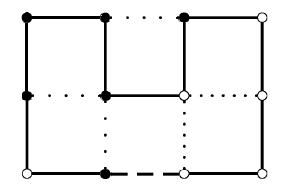
\includegraphics[scale=0.7]{figures/proteinExample.png}
	\caption{One possible configuration of  sequence $PPPPHPHHHHPH$ in the HP model. The white circles represents the P amino-acids and the black circles describes the H amino-acids. The sequence starts at the third white circle on the bottom of the figure. The next amino acids are positioned  counter-clockwise. There are two $H-H$ (represented by a dotted line with wide spaces), one $H-P$ (represented by a dashed line) and  two $P-P$  (represented by dotted lines) contacts. }
	\label{fig:PROTEXAM}
\end{figure}


%The total number of topological neighboring positions in the lattice ($z$) is called the lattice coordination number.


For the HP model, an energy function that  measures the amount of topological  neighbor residues is defined  as  $\epsilon_{HH}=-1$ and $\epsilon_{HP}=\epsilon_{PP}=0$. The HP problem consists of finding the protein configuration that minimizes the total energy. In the linear representation of the sequence, hydrophobic residues are represented with the letter H and polar ones, with P. In the graphical representation, hydrophobic proteins are represented  by black beads and polar proteins, by white beads.  Fig \ref{fig:PROTEXAM} presents a possible graphical conformation  of a sequence   in the 2D lattice. The energy associated with this conformation is $-3$. 


%Among many works that explores the PSP problem, here are some examples of the approaches that have been used to solve it.
We briefly review some of the previous studies on the optimization of the simplified PSP, relevant for our research.


%
%Alternative
%Unger and Moult \cite{unger1993genetic} described a genetic algorithm (GA) that uses heuristic-based operators for crossover and mutation for the HP model.


A study presented in \cite{krasnogor2002multimeme} introduces the MMA (Multimeme algorithm) which consisted on an EA combined with a
group of local search methods. For each individual in the population, the MMA selects the local search method that is more suitable with the individual. Used first to find solutions for the functional model protein, the strategy was later improved with fuzzy-logic-based local searches, leading the algorithm to achieve improved results in the PSP problem.

%The multimeme algorithm (MMA) proposed by \cite{krasnogor2002multimeme} is a GA combined with a set of local search methods. The algorithm, for each different instance or individual in the population, selects the local search method that best fits. 




%Originally used to find solutions for the functional model protein. The algorithm was later improved with fuzzy-logic-based local searches, leading the algorithm to produce improved results in the PSP problem.


In \cite{hsu2003growth}, Hsu et al. present the  pruned-enriched Rosenbluth method (PERM), also known as chain growth algorithm, that is based on growing the sequence conformation by adding particle by particle, aiming to increase good configurations and eliminating bad ones.


The ant colony optimization (ACO), in \cite{shmygelska2003improved}, was applied to the PSP problem using the HP-2D model. This strategy, uses artificial ants to build conformations for a given HP instance (sequence of amino-acids). A local search method is then applied to further improve the solutions and also maintain the quality of the solutions.

The study of Santana et al. \cite{santana2008component} applies EDAs as an efficient evolutionary algorithm that learns and exploits the regularities of the search space in the form of probabilistic dependencies. They introduced new probabilistic models tailored for the application of EDAs to 2D and 3D simplified protein folding problem. The obtained results showed that EDAs can achieve superior solutions compared with other well-known population based optimization algorithms.



%TODO: Multi Objective, maybe replace with another work, probably the Sabar one should be a good option here
%Gabriel \textit{et al}. \cite{gabriel2012algoritmos} propose the use of a table-based multi objective evolutionary algorithm initially introduced by \cite{delbem2002restabelecimento}, using the HP-3D model for the representation and solution evaluation. The authors also propose the use of a second objective that aims to measure the distance between hydrophobic amino-acids, allowing the algorithm to distinguish between different solutions with the same energy value.

%%TODO: check how to improve it
%The present paper proposes the use of a grammatical evolution GE to generate high level heuristics for a hyper heuristic framework that will be applied to the PSP problem.

%TODO: explicar que diferente heuristics foram propostas, como tentar combinar elas de maneira melhor utilizando hyper heuristica, explorando GE para gerar as heuristicas de alto nivel.
\section{Background}
\label{sec:background}

This section will present the background context in order to provide the readers with the necessary information, for a good comprehension of the concepts and techniques used in this paper.  


\subsection{Hyper-Heuristics}
\label{subsec:hyperheuristics}

%Hyper-Heuristics can be seen as a methodology to select or create heuristics for a given moment of the search. 
	Mainly, a generic hyper-heuristic framework is composed of two  components known as high-level and low-level heuristics. Fig \ref{fig:HyperHeuristicsImg} shows a general scheme of hyper-heuristic frameworks. The high and low levels are separated by a domain barrier which means that the low-level component is problem dependent while the high-level component does not require any knowledge of the problem domain. Ideally it is possible to apply a hyper-heuristic framework to a different problem domain by only replacing the low level component. The responsibility of a high-level component is manage the selection or generation of which heuristic should be applied at each decision point. The low-level component corresponds to a pool of heuristics or heuristic components \cite{sabar2012grammatical}. 
 
 
\begin{figure}[htb!] 
	\centering
	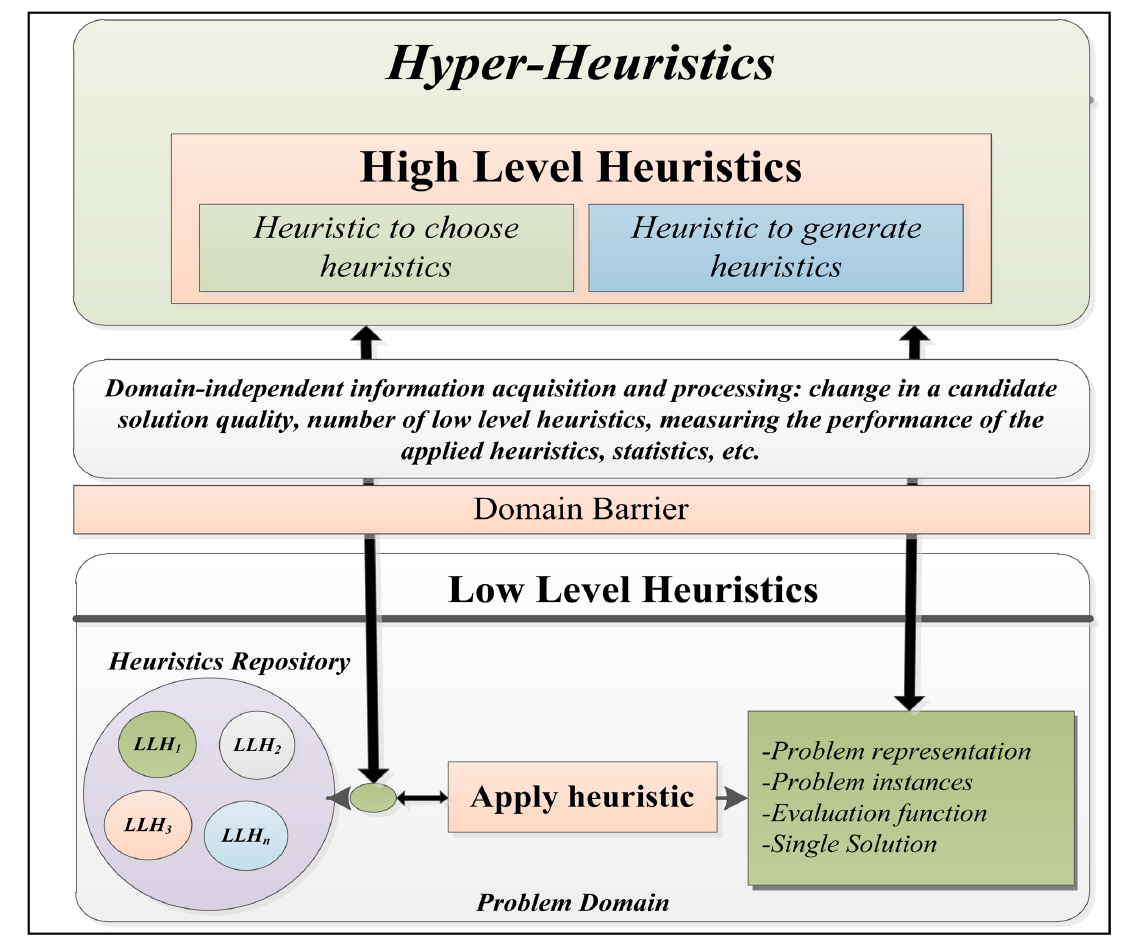
\includegraphics[scale=0.21]{figures/HH.png}
	\caption{General scheme of a hyper-heuristic framework \cite{sabar2012grammatical}.}
	\label{fig:HyperHeuristicsImg}
\end{figure}	



%Recently Burke et al. \cite{burke2010classification} classified hyper-heuristic frameworks based on the source of feedback during the learning process and the nature of the search space. In the case of the source of feedback Burke el al. \cite{burke2010classification} mention 3 possibilities: online, offline and no learning. If the hyper-heuristic framework uses information gathered during the problem solving it is considered as an online framework. An offline framework requires a training phase to gather information in order to use later in the validation phase. No learning occurs when no feedback is provided to the hyper-heuristic framework \cite{sabar2015automatic}. The nature of the search space can be either selecting or generating heuristics for the underlying problem. Next will be analyzed both kinds of high-level heuristics.


Based on the nature of the search space,  hyper-heuristics can be classified as either selecting or generating heuristics for the underlying problem \cite{burke2013hyper}. Next we analyse both types of high-level heuristics.


\begin{itemize}
	\item Selecting Heuristics: The majority of  hyper-heuristic frameworks define high level heuristics to select low level heuristics \cite{burke2013hyper}. In general, these frameworks define a selection mechanism and also an acceptance criterion. These strategies use information from the statistical history of low level heuristics applications. For instance, a greedy selection considers only the number of improvements that a low level heuristic obtained. In contrast, the choice function \cite{burke2013hyper} is a reward-based strategy, which considers both the number of improvements and the elapsed time since the last application.
	
	
%	Using statistical information (e.g: number of improvements, rewards , number of accepts, amount of improvement) related with the low level heuristics applications, the high level heuristics are made of.
	%TODO: maybe change to built out
	
	
	
	
	
	
	
%	The pool can contain both constructive or perturbative heuristics. 
%	
	
%	The objective of the hyper-heuristic framework is to select the heuristic, from the pool, which most suits at a given moment. The main idea behind this: the strength of several heuristics can be combined into a single framework in order to better explore the search space. 
%	Most of the proposed selection mechanisms use simple rules to select the low level heuristics based on their past performance \cite{sabar2015automatic}.

	\item Generating Heuristics: In this case, the hyper-heuristic framework starts with a set of subcomponents  from the low level heuristics and has the goal of building new low level heuristics with it. GP is reported as a good strategy to combine and generate new heuristics for the SAT, scheduling, and bin-packing problems \cite{burke2013hyper}.
\end{itemize}


%TODO: Mencionar que gera online dois componentens, criando selecao e aceitao,e o nosso é offline
%mencionar fase de treinamento e validacao
Two studies presented by Sabar et al. \cite{sabar2012grammatical,sabar2015automatic}, proposes an on-line approach to generate selection mechanisms and acceptance criteria (high level heuristics) to a hyper-heuristic framework. The results in both studies outperforms some bespoke strategies, which have reported best known results in some instances of the domain problems explored. This encouraging results inspired the present study which has the objective of generating selection mechanisms and acceptance criteria, through a grammatical evolution process in a off-line manner, for a hyper-heuristic framework to solve the PSP problem using the simplified HP-2D model.





\subsection{Genetic Programming {(GP)}}
\label{sec:geneticprogamming}
 It is a sub-field from program synthesis which uses ideas from evolution theory to produce programs \cite{koza1992genetic}. 

% The main factors from the evolutionary computation are inheritance, reproduction/mutation and selection of the fittest. Initially, a random-generated population of programs is created. Using a selection method to select good individuals for reproduction. Then the reproduction and mutation steps takes place in order to generate an offspring. Finally, the offspring is evaluated to assign a fitness value and based on this value the offspring can either enter or not in the population. 

%Traditionally, in genetic programming, the programs that compose the population are represented using a tree structure. However, other structures that can be evolved exists, for instance: linear sequences of instructions and grammar expressions. 

Grammatical Evolution (GE) is a relatively new technique from the evolutionary computing, introduced by Ryan el al. \cite{ryan1998grammatical} and it is a type of GP where programs are evolved using a genetic algorithm. The chromosome encodes production rules of the grammar. GE uses a mapping mechanism between the genotype (coded individuals by integer vectors) and phenotype (generated programs to solve a problem). The BNF notation is used to represent a grammar from a language in the form of production rules. A BNF grammar consists in a set of terminals, which are items that are allowed in the language, for instance: +, -, *, /, etc and non-terminals, which can be expanded into one or more terminals. The Grammar can be expressed as a tuple ${N,T,P}$, where $N$ is a set of non-terminals presented in the Grammar \ref{gram:gramatica} as $\langle expr \rangle$, $\langle op \rangle$, $\langle pre - op \rangle$ and $\langle var \rangle$,  $T$ a set of terminals and is presented in the Grammar \ref{gram:gramatica} as $+$, $-$, $/$, $*$, $Sin$, $Cos$ and $Tan$. Finally, $P$ is the set of production rules that maps the elements $N$ to $T$ and is presented in Table \ref{tab:productionRules}.

%TODO: Explicar tudo N,T,P,S com grammar um e remover expressao


%Just like in GP the main goal is to find a executable program or piece of code, which have a good fitness value. 
%
%
%Ryan el al. \cite{ryan1998grammatical} proposes a technique to generate programs or fragments for any language using BNF (Backus Naur Form) definitions. This technique can be used to evolve programs though a evolution process. 

%\begin{center}
%	
%	$ N = {\langle expr \rangle, \langle op \rangle, \langle pre-op \rangle}$
%	
%	$ T = {Sin,Cos,Tan,Log,+,-,/,*,X} $
%	
%	$ S = \langle expr \rangle $
%	
%\end{center}

%\noindent
%And $P$ is presented by the Grammar \ref{gram:gramatica}:

\begin{Grammar}

	\begin{grammar}
		
		
		<expr> :=  <expr> <op> <expr> \hspace{2cm} (0) 
		\alt (<expr> <op> <expr>)  \hspace{1.75cm}  (1)  
		\alt <pre-op> (<expr>) \hspace{2.2cm}  (2) \alt <var> \hspace{3.9cm} (3) \\\
		
		<op> :=  + \hspace{4.4cm} (0)   \alt - \hspace{4.5cm}  (1)  \alt  /  \hspace{4.51cm}  (2) \alt * \hspace{4.45cm}  (3) \\
		
		<pre-op> := Sin \hspace{4.2cm} (0) \alt Cos
	\hspace{4.12cm} (1) \alt Tan  \hspace{4.13cm} (2) \\
		
		<var> := X  \hspace{4.4cm} (0)
		
		
	\end{grammar}
	
	\caption{Sample grammar to demonstrate how to decode integer vectors in computer programs}
	\label{gram:gramatica}
\end{Grammar}


\begin{table}[htb]
	\centering
	\caption{Example of Possible Production rules and the number of choices allowed}
	\label{tab:productionRules}
	\begin{tabular}{|l|l|}
		\hline
		Production Rules & Number of choices \\ \hline
		$\langle expr \rangle$                        & 4       \\ \hline
		$\langle op \rangle$                         & 4       \\ \hline
		$\langle pre-op \rangle$                         & 3       \\ \hline
		$\langle var \rangle$                          & 1       \\ \hline
	\end{tabular}
\end{table}


	Ryan et al. \cite{ryan1998grammatical}  proposed the use of a GA to control which choices should be made, in this sense allowing the GA to select which production rules should be utilized. Algorithm \ref{alg:GE} presents the pseudocode of a grammatical evolution program. Lines 3 to 6 represent the initialization of the algorithm: a randomly generated population is created and then mapped to programs using the GF (Grammar File). Those programs are evaluated and a fitness value is assigned for each individual in the population. Line 7 indicates the start of the main loop of the algorithm and the evolution process occurs within this loop. Line 8 invokes the parent selection that will be used in the crossover in Line 9 which will generate an offspring (integer vectors). The offspring is then used as input to prune and duplication operators in Lines 10 and 11. The mutation operator is applied to the offspring in Line 12. The mapping between the integer vectors to programs is accomplished in Line 13. Next the execution and fitness assignment to the individuals from the population are implemented in Line 14 and 15. The population replacement with the fittest individuals is done in Line 16. Finally, Line 18 returns the program with the best fitness found.
 
\begin{algorithm}[htb]
	\fontsize{6pt}{8pt}\selectfont
	\caption{Pseudo code from the Grammatical Evolution}
	\label{alg:GE}
	\KwIn{GF -- Grammar File}
	\Begin{
		$population \gets$ Create population\;
		$programs \gets$ Maps the $population$ to programs using $GF$\;
		Execute the $program$\;
		Assign fitness value with the solutions of $population$ according with the output obtained by the respective decoded program\;
		\While{Stop condition not reached}{
			$parents \gets $ Select individuals for crossover\;
			$offspring \gets$ Crossover($parents$)\;					
			Apply the \textit{Prune} operator to the $offspring$\;
			Apply the \textit{Duplicate} operator  to the $offspring$\;
			Apply the \textit{Mutation} operator to the $offspring$\;
			$programs \gets$ Maps $offspring$ to programs using $GF$\;
			Execute $programs$\;
			Assign \textit{fitness} value to $offspring$ according with the output obtained by the respective decoded program\;
			$population \gets$ Replacement\;
		}
		\Return{Best program from the $population$}\;
	}
\end{algorithm}

Algorithm \ref{alg:pseudocodigogrammar} presents the general template of the generated programs. In Line 3 the variable $f$ receives a function returned by the genotype/phenotype mapping. The function is executed and the resulting value is returned in Lines 4 and 5.


\begin{algorithm}
	\caption{General template for the generated algorithms}
	\fontsize{6pt}{8pt}\selectfont
	\label{alg:pseudocodigogrammar}
	\KwIn{int[] chromossome;}
	\Begin{
		Function f = mapGenotypeToPhenotype(chromossome);\\
		double value = f.execute();\\	
		\Return value;  \\
	}
		
\end{algorithm}


% TODO: SHOULD BE USED IN THE METHODOLOGY IF 
%\begin{algorithm}
%	\caption{General template for the generated algorithms}
%	\fontsize{8pt}{10pt}\selectfont
%	\label{alg:pseudocodigogrammar2}
%	\KwIn{chromossome -- Integer[], selectionMechanismFixed SelectionMechanism, acceptanceFunctionFixed AcceptanceCriterion}
%	\Begin{
%		SelectionMechanism selectionMechanism; \\
%		AcceptanceCriterion acceptanceCriterion;
%		\If{config.isSelectionGenerationEnabled}
%		{selectionMechanism = ChromossomeUtils.mapToSelectionFunction(chromossome);}
%		{selectionMechanism = selectionFunctionFixed;}
%		
%		\If{config.isAcceptanceGenerationEnabled}
%		{acceptanceCriterion = ChromossomeUtils.mapToAcceptanceCriterion(chromossome);}
%		{acceptanceCriterion = acceptanceCriterionFixed;}
%	}
%
%	float symb() { \\
%		a = $\langle expr \rangle$;   \\s
%		return a;  \\
%	}	
%\end{algorithm}


\noindent

The mapping process to decode a genotype on its phenotype will be demonstrated using the following integer vector:

\begin{center}
	$ [220, 203, 17, 6, 108, 215, 104, 30] $
\end{center}

This vector will be used to decode the chromosome (genotype) into a piece of code (phenotype)  using the Grammar \ref{gram:gramatica}.
Table \ref{tab:productionRules} summarizes the number of choices associated within each production rule from Grammar \ref{gram:gramatica}. 

There are 4 options of production rules that can be selected for the expression $ \langle expr \rangle$. In order to determine which is the option to select, the first value from the vector should be used. The value is 220 and its remainder divided by 4 (four options that can be selected for the expression $ \langle expr \rangle$) results in 0, which means that the first option should be selected $\langle expr \rangle \langle op \rangle \langle expr \rangle$. Note that the first expression is also $ \langle expr \rangle$ and following the same logic we should expand using the next value from the integer vector and apply its remainder by the division of the number of options. The remainder of 203 $\%$ 4 = 3, which indicates that we should select the fourth option: $ \langle var \rangle$ which is a terminal. The $ \langle var \rangle$ has just one option associated with it and is the value $X$. Placing this selection in the original expression we have $X \langle op \rangle \langle expr \rangle$. 

Next, it is necessary to decode the non-terminal expression $\langle op \rangle$. The next value from the integer vector is 17 and again we have 4 options $(+ | - | / | *)$. The result is equal to 1, and indicates to select the: $-$. Re-writing the expression we got:  $X  -  \langle expr \rangle$. This process should continue until all the non-terminals have been expanded to terminals. In this example the resulting expression (phenotype) is: $X - sin (X)$. Note that not all of the genes were necessary to obtain the phenotype. In these cases, the genes that were not used are discarded. Moreover, the opposite case can occur: if a chromosome does not contain the necessary number of genes to map to a program. In this scenario the strategy is to re-use the genes starting from the first one.

%O Algoritmo \ref{alg:GE} apresenta o pseudocódigo da evolução gramatical (EG). Note que o pseudocódigo é muito similar a um algoritmo genético simples. Nas linhas 3 e 4 ocorre a inicialização da população e o mapeamento para programas utilizando a gramática que foi provida como entrada. Em seguida, na linha 5 ocorre a execução dos programas e na linha 6 acontece a avaliação dos indivíduos da população, baseando-se na saída obtida pelos respectivos programas. Dentro do laço principal, apresentado na linha 7, podemos observar o processo de seleção dos indivíduos pais na linha 8 e na linha 9 o processo de cruzamento destes indivíduos. Nas linhas 10 e 11 ocorre a aplicação dos operadores \textit{Prune} e \textit{Duplicate} respectivamente e na linha 12 podemos observar a aplicação do operador de mutação. Em seguida, nas linhas 13,14 e 15 ocorre o mapeamento dos indivíduos descendentes para programas, execução dos programas e finalmente a atribuição de \textit{fitness} para os descendentes. Por fim, na linha 16 do laço principal, ocorre a substituição dos descendentes na população. 


%exceto pela aplicação dos operadores \textit{Duplicate} e \textit{Prune} (linhas 10 e 11 do Algoritmo  \ref{alg:GE}) e o processo de decodificação e execução dos programas descendentes (linhas 13 e 14 do Algoritmo \ref{alg:GE}).


%TODO: check if this will be needed
%\section{Genetic Programming as Hyper-Heuristic to Generate Heuristics}
%\label{subsubsection:PGasHH}
%
%In this section will be presented how GP/GE can be used as mechanism to generate heuristics. Burke et al. \cite{burke2009exploring} describes that many authors mentioned the great suitability of GP to automatically generate new heuristics. Burke et al. \cite{burke2009exploring} also describes some advantages of using this technique. 
%
%\begin{itemize}
%	\item GP uses variable-length chromosomes. Usually, is not possible to define a ideal length to represent heuristics from a given domain problem. 
%	\item GP produces executable data structures and heuristics 
%	usually are expressed as programs or algorithms.
%	\item Ease to identify good characteristics from the problem domain in order to define a terminal set which will be used by the GP.
%	\item Human designed heuristics can be easily expressed in the same language used to create the search space from the GP. The function set, relevant from the problem can be easily determined. Additionally the GP can be supported by a specific grammar which is the case of the GE.
%\end{itemize}
%
%These advantages presented by Burke et al. \cite{burke2009exploring} are also characteristics from the GE, since it is a extension from genetic programming and holds the same features (variable-length, produces executable structures, etc).
%
%Some disadvantages are also described by Burke et al. \cite{burke2009exploring}, for instance: each execution of the GE can return different results because its stochastic behavior. Thus, it is necessary to execute multiple times, in order to obtain a better understanding of the quality from the heuristics that can be achieved. Another disadvantage refers to the parameter configuration, which is usually found by trial and error.

%
%\subsubsection{Basic Approach}
%
%Burke et al. \cite{burke2009exploring} also describes a basci approach to apply genetic programming to generate heuristics.
%
%
%\begin{enumerate}
%	\item Review of the existing heuristics: Analyze if
%	the already proposed heuristics for a given problem can be described into a single framework. These heuristics can be human made or even created by other machine learning techniques. This is step is not trivial, it requires a good understanding of a wide range of existing heuristics. Usually human-designed heuristics are products from years of research. Therefore, a good knowledge of the existing heuristics can be a tough work.  	
%	
%	\item A framework which will use the heuristics: At this moment the concern is how the heuristics will be applied for a given problem. Usually, the frameworks tends to be very different depending on the problem.
%	 
% 
%	\item Terminal set definition: At this step the concern is the variables that express the state of the problem. These variables will compose the terminals from the GP/GE. Also, other terminals can be used for instance: random constants can be useful.
%	
%	\item Function set definition: It is necessary to define how the variables will be related or combined each other. These relationships will compose the function set of the GP/GE.
%
%	\item Fitness function definition: A fitness function should be identified for the problem. Usually, a simple fitness function will not be able to evaluate properly the chromosomes. Inserting some parameters can help to find the most suitable function.
%	
%	\item Framework execution: Usually, in the first execution of the hyper-heuristic framework the results will not achieve good results, mostly due the parameter configuration. This is observed especially when the research is beginner. Therefore, it is essential that the parameter configuration be carefully investigated.
%
%\end{enumerate}


\section{GEHyPSP}
\label{sec:methodology}
This section presents GEHyPSP: an off-line grammatical evolution application for generating the high level heuristics of a hyper-heuristics framework for the Protein Structure Prediction problem. Our approach is based on the study by Sabar et al. \cite{sabar2012grammatical}



%This paper explores grammatical evolution instead of gene expression programming and also it executes, in a different domain problem, using the PSP within HP-2d model. 



%According to Krasnogor et al. \cite{krasnogor1999protein}  the relative representation have a better potential to achieve superior results. 


%This representation was used to represent the chromosome within the PSP and the HP-2d model and will be explained next: the movements in the grid for each amino-acid are represented always based on the previous, that is why the representation is named relative. There are 3 possible movements within the HP-2d model: forward (F), left (L) and right (R). Hence, the following integer codification was used $F\rightarrow0$, $E\rightarrow1$ and $D\rightarrow2$. Thereby, the allowed alphabet can be represented as $\{0,1,2\}$.


 The high level heuristics are composed of a selection mechanism and an acceptance criterion. These high level heuristics use information related of the history of low level heuristics applications. Data about the improvements obtained by the low level heuristics, number of times since the last application of a low level heuristic and the fitness difference between the current solution and the generated one are examples of information used by selection mechanisms and acceptance criteria.  Furthermore, two terminal sets (one for the selection mechanisms and another for the acceptance criteria) were defined according to the information that can be extracted during the search progress. The selection terminals are:

%:TODO: Paragrafao explicando que a GEHyPSP irá gerar dois main components e tirar o as mentioned
%As mentioned on Sub-section \ref{subsec:hyperheuristics} the selection mechanisms and acceptance criterion uses information related with the history of low level heuristics applications.
%TODO: explicar que informacoes são, para criar bons criterios eu tenho que levar em consideracao informacoes relativas ao execucao das low level heuristics. Convencer o usuario que esse é um bom terminal set. Explicar oque é importante para um mecanismo de seleção. e Outro paragrafo para critério de aceitacao.



\begin{itemize}
	\item RC (\textit{Reward Credit}): The reward that a given heuristic should receive based on its performance. The improvement is calculated, for the $i_{th}$ heuristic, using $M(i) = (|f1 -f2|/f1)*100$ if $f2< f1$, where $f1$ is the current fitness and $f2$ is the fitness of the solution generated by the $i_{th}$ heuristic.
	
 	\item $C_{best}$: Number of times that the $i_{th}$ heuristic updated the best known solution. 

	\item $C_{current}$: Number of times that the $i_{th}$ heuristic updated the current solution. 

	\item $C_{accept}$: Number of times that the solution generated
	by the $i_{th}$ heuristic was accepted by the acceptance criterion.

	\item $C_{ava}$: The average of previous improvements made by the $i_{th}$ heuristic during the search progress.
	\item $C_r$: Number of times that the $i_{th}$ heuristic was selected to be applied.
	
	\end{itemize} 

A specific terminal set for generating acceptance criteria was also defined.


 \begin{itemize}
 	 \item Delta: The difference between the quality of the current solution and the generated solution.
 	\item PF: The quality of the previous solution.
 	\item CF: The quality of the current solution.
 	\item CI: Current iteration of the search progress.
 	\item TI: Total number of iterations of the search progress.
 \end{itemize}
	 
  Using these statistics as terminals and a function set containing the following arithmetic operations: addition, subtraction, multiplication and division, a grammar was designed. The Grammar \ref{grammar:proposedGrammar} presents an BNF notation to represent the grammatical rules. Within these rules it is possible to generate arithmetic functions. These functions can be applied to sort the low level heuristics set. When a low level heuristic is ranked first, this heuristic is selected to be applied generating the next solution. In the same way, the acceptance criterion will accept solutions only if the outcome obtained by the acceptance arithmetical function is higher than 0.5.
  
 

 For the initialization of the terminal set data: all heuristics were executed once and the data for each terminal was computed. Every consecutive iteration will update the terminal set data and this information will be used during the search.
 

 \begin{Grammar}
 	
 	\begin{grammar}
 		
 		<hh-selection> ::= <selection-mechanism> <acceptance-criterion> 
 		
 		<selection-mechanism> :==  <selection-terminal>   
 		\alt <selection-mechanism> <math-function> <selection-mechanism> 
 		\alt (<selection-mechanism> <math-function> <selection-mechanism>) 
 		
 		<selection-terminal> :== 
 		RC 
 		| Cbest 
 		| Ccurrent 
 		| Caccept 
 		| Cava 
 		| Cr
 		
 		<math-function> :== + 
 		| - 
 		| * 
 		| \%
 		
 		<acceptance-criterion> ::== <acceptance-terminal> 
 		\alt <acceptance-criterion> <math-function>
 		<acceptance-criterion>
 		\alt (<acceptance-criterion>  <math-function> <acceptance-criterion>) 
 		
 		<acceptance-terminal> :== PF | CF | CI | TI
 		
 		%	<acceptance-function> :== + | - | * | \% | $e^x$
 		
 		
 	\end{grammar}
 	\caption{Designed grammar to generate high level heuristics}
 	\label{grammar:proposedGrammar}
 \end{Grammar}

%Using the Grammar \ref{grammar:proposedGrammar} and integer vectors is possible to generate high level heuristics. The terminal sets from the grammar presents statistic information from the history of  the low level heuristics application. This information is used as raw material for building the selection mechanisms and the acceptance criteria to a hyper-heuristic framework.
%
%The next step consists of evolving a population of integer vectors, initially random generated, using the evolution process described in Sub-section \ref{sec:geneticprogamming}. 
\subsection{Fitness Function to evaluate the High Level Heuristics}
\label{subsection:fitnessFunction}


In order to evaluate the individuals generated during the search, a fitness function was designed. The fitness function consisted of running the generated high level heuristics, within a hyper-heuristic framework, on three random selected instances from a set of eleven instances. The motivation behind executing the high level heuristic (individual) against three HP instances is that executing with only one might not be sufficient to train a high level heuristic to obtain good results for various instances of the HP model.
	
	Each run will be executed for 30 minutes and will return the best HP solution found. The fitness value associated with the returned solution is then normalized between 0 and 1. The fitness of an individual, of the GE, is the sum of the three outcomes from each execution of the three randomly selected instances. Hence, the best possible fitness value is 3 and the worst is 0.






%In order to evaluate the generated individuals during the search progress, a fitness function was designed based on the Sabar et al. \cite{sabar2015automatic} work. The probability of selecting an individual, changes according to the quality of the best solution returned by the execution of the hyper-heuristic framework using the high level heuristics coded by the individual. 
%
%Suppose that $f_i$, $f_o$ represents respectively the quality of the input and output solution and $P_h$ the vector of probabilities of selecting the individuals from population. Now suppose that when applying the $i_{th}$ individual and it obtained an improvement the reward will be calculated using Equation \ref{eq:fitnessFunction}.
%
%\begin{equation} {}
%\label{eq:fitnessFunction}
%Ph[i] = Ph[i] + \sigma 	
%\end{equation} 
%
%Where $\sigma = (f_i - f_o)/(f_i + f_o)$. 
%
%And all other individuals  $j \neq i$ should be penalized using Equation \ref{eq:fitnessPenalizeFunction}
%
%\begin{equation} {}
%\label{eq:fitnessPenalizeFunction}
%Ph[j] = Ph[j] - (\sigma / (Nh - 1))
%\end{equation}
%
%Such that  $j \in \{1, ..., Nh\} ~e~ j \neq i$. And $Nh$ the number of individuals.
%
%Otherwise (if the output solution is worst than the input), a penalization should be applied to the $i_{th}$ individual using Equation \ref{eq:fitnessBadFunction}.
%
% \begin{equation} {}
% \label{eq:fitnessBadFunction}
% Ph[i] = Ph[i] - |\sigma \times \alpha|
% \end{equation}
% 
% Where $\alpha =$ current iteration $/$ total number of iterations.
% 
% And all other individuals $j \neq i$ should receive a reward using Equation \ref{eq:fitnessOtherFunction} 
% 
% \begin{equation} {}
% \label{eq:fitnessOtherFunction}
% Ph[j] = Ph[j] + (|\sigma| \times \alpha / (Nh -1))
% \end{equation}
% 
% Such that  $j \in \{1, ..., Nh\} ~e~ j \neq i$. Where $Nh$ = number of individuals and $\alpha =$ current iteration $/$ total number of iterations.
% 
% The motivation behind decreasing the probability from the other individuals is to reduce the chances of those individuals to be selected. Initially, the probability os each individual is calculated, decoding the respective selection mechanism and acceptance criterion and executing it within a hyper-heuristic framework for a defined number of iterations.
%  
\subsection{Stopping Criterion}
\label{sub:criterioParada}

To stop the GE process, a maximum number of evaluations was setup to 60000. This value was defined based on previous work \cite{ryan1998grammatical} where the grammatical evolution general process was introduced for the first time. 

  \subsection{Low Level Heuristics} 
  
  \subsubsection{Representation of the problem} 
  There are many ways of representing a protein conformation within the HP-2D model. According to Krasnogor et al. \cite{krasnogor2002multimeme}  the relative representation has a better potential to achieve superior results. The relative representation defines that each gene of the chromosome represents a direction in the grid. Each gene will encode an conformation that a protein could adopt.
  The directions in the grid for each amino-acid are represented always based on the previous one. There are 3 possible directions within the HP-2D model: forward (F), left (L) and right (R). Hence, the following integer codification was used $F\rightarrow0$, $L\rightarrow1$ and $R\rightarrow2$. Thereby, the allowed alphabet can be represented as $\{0,1,2\}$.  

  \subsubsection{Low Level Heuristics Set}
% todo: put the other works
 The low level heuristics set was selected from previous studies \cite{benitez2015algoritmo,custodio2014multiple} that explore the PSP. The implemented low level heuristic set have 6 heuristics with different characteristics. The majority of the heuristics are applied to a single solution. However, there are cases that the heuristics require two individuals. In this cases the current solution and a second solution, randomly selected from the memory mechanism (See subsection \ref{subsubsection:memoryMechanism}), are used.  
 
 The low level heuristic set consisted  of the following:
 
  \begin{itemize}
  	\item \textit{Two Points Exchange} (2X): This heuristic selects, randomly, two exchange points from two individuals. The genes between the selected positions are exchanged between the input solutions in order to generate a new one \cite{benitez2015algoritmo}. 
  	
  	\item  \textit{Multiple Points Exchange} (MPX): Similar to 2X although with $c$ points of exchange. We use $c=int(n*0.1)$, where $n$ is the instance length. The MPX is useful to promote a wide structural diversity \cite{sabar2015automatic}.
  	
	\item \textit{Segment Change} (SG): Given an individual it changes multiple consecutive genes, between 5 to 7, to distinct values. This heuristic introduces large changes in the protein conformation, and it has a great probability of creating collisions (cases in which the protein conformation are not self avoiding).  

	\item \textit {Exhaustive Search Change} (ESC): 	This heuristic selects a random gene of an individual and modifies it to other possible value. All possible values are tried and the one that achieved the higher improvement will be kept. 
	
	\item \textit{Local Move Operator} (LM): This heuristic exchanges directions between two consecutive random selected genes of an individual. This heuristic introduces small local changes that can reduce the distance between pairs of H-H.
	
	\item \textit{Loop Move Operator} (LPM): Similar with LM, this heuristic exchanges directions between two genes that are five genes of distance between each other.
	
	
	\item \textit{Opposite Change} (OC): This heuristic exchanges multiple genes between two points $(i,j)$, of an individual, to the respective opposite. In the HP-2D this means that genes that code L are changed to R or vice and versa. The F has no opposite thus, the operator is not applied. 

 \end{itemize} 

 This low level heuristic set will be used by the generated high level heuristics. In other words the selection mechanisms have the responsibility of selecting the most suitable heuristic for each iteration.
 
 \subsubsection{Backtrack Repair}

The low level heuristics have a great potential of creating solutions with collisions \cite{benitez2015algoritmo}. Those solutions are submitted to a repair procedure that uses a backtrack strategy. The solutions that can be repaired are kept and the others are penalized. 
 


\subsubsection{Memory Mechanism}
\label{subsubsection:memoryMechanism}
Sabar et al. \cite{sabar2012grammatical} suggested that the use of a memory of solutions to the PSP would be more effective. Relying with a single solution. may restrict the ability of dealing with large and heavily constrained search spaces.



\section{Experiments}
\label{sec:experiments}

%Mencionar que é comparado GIHH  e explicar o GIHH.

In this section, we will present and discuss the conducted experiments in order to evaluate GEHyPSP performance. Since GEHyPSP is an offline strategy the experiments are divided in two phases: training and validation. The training phase consisted o executing the GEHyPSP to search for high level heuristics that can achieve good results for the fitness function described in \ref{subsection:fitnessFunction}. The validation phase consisted on executing the best individuals found in the training phase and execute again but now against all instances. Unfortunately, the results of the training phase were suppressed from the paper because of space limitations. Only the results of the best individuals found are presented.


Three groups of experiments were designed/executed. The first group was only concerned on generating selection mechanisms. The second group was designed only to generate acceptance criteria. The third group was developed to generate both selection and acceptance mechanisms. All experiments were executed 30 times because of the stochastic behavior of the GEHyPSP. 


The results obtained by the groups were first compared with each other. Next, the results were compared with the best known results. Also a final comparison was made with a state-of-art hyper-heuristic. The proposed strategy was compared with the Generic Intelligent Hyper-heuristic (GIHH) presented by Misir el al \cite{misir2012intelligent}.



In the first group of  experiments (GEHyPSP-1), only selection mechanisms are generated. The acceptance criterion was fixed with a "better or equal" acceptance \cite{burke2013hyper}. This strategy only accepts (replace the current solution) the generated solution if its fitness is better or equal than the current solution.

The goal of this group is to evaluate the ability of our approach to generate selection mechanisms using a fixed and human-designed acceptance criterion.   

The second group of experiments, GEHyPSP-2, consisted on  generating only acceptance criteria. The selection mechanism was fixed using the best selection mechanism found in the first group. Consequently, this group of experiments depends on the output from the first group. The goal of this experiment was to evaluate the generation of acceptance criteria separately from the selection mechanism using a fixed one.


% Fixing the selection mechanism, within the hyper-heuristic framework, with the better (the one with higher fitness from the 30 executions) selection mechanism generated by the GEHyPSP-1.  

%Quer avaliar entao a geracao conjunta dos dosi mecanimos
The third group of experiments GEHyPSP-3 was designed to  generate both selection mechanisms and acceptance criteria. The goal of this group was to evaluate the ability of generating selection mechanisms along with acceptance criteria. Differently from GEHyPSP-2, this group of experiments does not depend on any output from previous experiments since it generates both mechanisms without fixing any component.

%TODO: mencionar na tabela final que a aurora falou para colocar por ultimo
%Table \ref{tab:geExps} summarizes the average, standard deviations, max and min fitness values from 30 executions from the tree experiments.


For each group of experiments, eleven instances, selected from the literature, were used. The sizes (number of residues) of the HP instances used in the experiments are presented in Table \ref{tab:instances}. 
 For the sake of space, the sequences are not reproduced here. They can be obtained in \cite{santana2008component}. 


\begin{table}[]
	\centering
	\caption{Instances and the respective size of each one}
	\label{tab:instances}
	\begin{tabular}{cccccccccccc}
		Inst & 1 & 2 & 3 & 4 & 5 & 6 & 7 & 8 & 9 & 10 & 11 \\ \hline
		Size & 20 & 24 & 25 & 36 & 48 & 50 & 60 & 64 & 85 & 100 & 100 \\ \hline
	\end{tabular}
\end{table}



%TODO: Novo paragrafo cada um dos grupos rodados em base de treinamento e que depois os melhores individuos foram rodados, e explicar conjunto. Mencionar o tamanho das sequencias e tal

%TODO: BOtar sutitulo resultados grupo 1

%TODO: Tabela dois vai para o final discussao...
%\begin{table}[]
%	\centering
%	\caption{Average, Std Dev, Max and Min values of the 30 executions of the GEHyPSP experiments}
%	\label{tab:geExps}
%	\begin{tabular}{lllll}
%		& GEHyPSP-1 & GEHyPSP-2 & GEHyPSP-3 &  \\ \cline{1-4}
%		Average & 2,248  & 2,281  & 1,997  &  \\ \cline{1-4}
%		Std Dev & 0,117  & 0,160  & 0,152  &  \\ \cline{1-4}
%		Max     & 2,433  & 2,453  & 2,310  &  \\ \cline{1-4}
%		Min     & 2,001  & 1,894  & 1,847  & 
%	\end{tabular}
%\end{table}

%Considering that the range of the fitness can vary from 0 to 3, as described in Sub-section \ref{subsection:fitnessFunction} it is possible to see looking Table \ref{tab:geExps} that the GEHyPSP-1 and GEHyPSP-2 obtained higher average values in relation to GEHyPSP-3. The Kruskal and Wallis showed statistical difference between GEHyPSP-1 x GEHyPSP-3  and GEHyPSP-2 x GEHyPSP-3 but not between GEHyPSP-1 x GEHyPSP-2.

%This indicated that generating the high level heuristics separately was more effective instead of generating both. The GEHyPSP-1, GEHyPSP-2 and GEHyPSP-3 was executed to evolve the high level heuristics using only three instances from the PSP problem as training phase. 

\subsection{Results from GEHyPSP-1}

The best individual found in the GEHyPSP-1 was the following selection mechanism:  $RC * Ccurrent * Cava - Cr$ and it was executed 30 times with a time limit of 30 minutes against the eleven instances. Table \ref{tab:gexp1best}  presents the fitness average, standard deviation, minimum and maximum of 30 executions of the best individual found in the GEHyPSP-1 experiment. The last row denoted with O(x*) is the best known value for each instance. Analysing the last two rows it is possible to notice that only in 7 instances the selection mechanism generated achieved the best known results. However in case of instances 7, 9, 10 and 11 the results obtained are very far from the best known results.

%TODO: resultado grupo 1
\begin{table}[]
	\centering
	\caption{Results from the best individual found in GEHyPSP-1}
	\label{tab:gexp1best}
	\resizebox{\columnwidth}{!}{%
\begin{tabular}{cccccccccccc}
	Inst  & 1   & 2    & 3   & 4    & 5    & 6   & 7   & 8    & 9    & 10   & 11   \\ \hline
	Avg   & 8.1 & 7.6 & 6.7 & 11.9 & 17.4 & 16  & 30  & 28.3 & 40.1 & 35.6 & 35.9 \\ \hline
	St Dv & 0.3 & 0.5  & 0.5 & 0.7  & 1    & 1.4 & 1.7 & 2    & 2.7  & 2.1  & 2.9  \\ \hline
	Min   & 8   & 7    & 5   & 11   & 15   & 13  & 25  & 23   & 34   & 32   & 27   \\ \hline
	Max   & \textbf{9}   & \textbf{9}    & \textbf{8}   & \textbf{14}   & \textbf{23}   & \textbf{21}  & 33  & \textbf{42}   & 46   & 40   & 41   \\ \hline
	O(x*) & \textbf{9}   & \textbf{9}    & \textbf{8}   & \textbf{14}   & \textbf{23}   & \textbf{21}  & \textbf{36}  & \textbf{42}   & \textbf{53}   & \textbf{48}   & \textbf{50}
\end{tabular}
}
\end{table}

\subsection{Results from GEHyPSP-2}

The best individual found in the GEHyPSP-2 was the following acceptance criterion:  $( ( TI / Delta ) / ( ( Delta * ( ( TI / Delta ) / CI ) * Delta / Delta * TI ) - CI ) )$ and combined with the best individual from the GEHyPSP-1 the hyper-heuristic framework was executed 30 times for each one of the eleven instances with a time limit of 30 minutes. Table \ref{tab:gexp2best} presents the results of the best generated acceptance criterion by GEHyPSP-2 with the best selection mechanism generated in GEHyPSP-1. Again, looking at the two last rows it is possible to notice that the hyper-heuristic framework, using the best generated selection mechanisms and acceptance criterion, was not able to reach the best known results for many cases. And comparing Tables \ref{tab:gexp1best} and \ref{tab:gexp2best} it is possible to visualize that the results obtained by the GEHyPSP-2 are very far from the ones obtained by the first GEHyPSP-1. This means that the acceptance criterion was not able to achieve superior results than the acceptance criterion used in the GEHyPSP-1. The results achieved in the first experiment are very superior.





\begin{table}[]
	\centering
	\caption{Results from the best individual found in GEHyPSP-2
		}
	\label{tab:gexp2best}
	\resizebox{\columnwidth}{!}{%
	\begin{tabular}{cccccccccccc}
		Inst  & 1   & 2   & 3   & 4    & 5    & 6    & 7   & 8    & 9    & 10   & 11  \\ \hline
		Avg   & 8   & 7.6 & 6.7 & 10.1 & 14.8 & 14.7 & 27  & 25.7 & 38.3 & 32.8 & 30. \\ \hline
		St Dv & 0.6 & 0.4 & 0.6 & 0.7  & 1.5  & 1.4  & 2.0 & 2.5  & 3.3  & 3.7  & 3.4 \\ \hline
		Min   & 7   & 7   & 5   & 8    & 12   & 12   & 23  & 22   & 31   & 26   & 24  \\ \hline
		Max  & \textbf{9}   & 8   & \textbf{8}   & 11   & 17   & 18   & 31  & 31   & 44   & 40   & 37  \\ \hline
		O(x*) & 9   & 9   & 8   & 14   & 23   & 21   & 36  & 42   & 53   & 48   & 50 
	\end{tabular}
}
\end{table}

\subsection{Results from GEHyPSP-3}

The best individual generated by the experiment GEHyPSP-3 was both a selection mechanism and an acceptance criterion. And they are presented below: \\ 
Selection Mechanism: $( ( ( ( ( Caccept / RC ) * Cr / Caccept ) / RC * Cr ) / Caccept / RC ) * Cr ) / Caccept$ \\
Acceptance Criterion: $( ( ( ( ( CI / PF ) * Delta / CI ) / PF * Delta ) / CI / PF ) * Delta ) / CI$

Table \ref{bestGExp3} presents the results of the best individual generated by the experiment GEHyPSP-3, of 30 executions with a time limit of 30 minutes. Once again the values presented did not achieve good results for most instances. Only for 2 very simple instances the best known results were achieved. Consequently, when comparing Table \ref{bestGExp3} with Tables \ref{tab:gexp1best} and \ref{tab:gexp2best} it is possible to see that generating both selection mechanisms and acceptance criteria produces worse results than generating them separately.

\begin{table}[]
	\centering
	\caption{Results from the best individual found in GEHyPSP-3}
	\label{bestGExp3}
	\resizebox{\columnwidth}{!}{%
		\begin{tabular}{cccccccccccc}
			Inst  & 1   & 2   & 3   & 4   & 5    & 6    & 7   & 8    & 9    & 10  & 11   \\ \hline
			Avg   & 7.6 & 7.0 & 5.7 & 9.7 & 13.8 & 12.7 & 24  & 24.2 & 31.6 & 27  & 26.4 \\ \hline
			St Dv & 0.6 & 0.7 & 0.8 & 0.9 & 1.3  & 0.9  & 1.1 & 1.6  & 1.7  & 1.7 & 2    \\ \hline
			Min   & 7   & 6   & 4   & 7   & 12   & 11   & 21  & 21   & 29   & 24  & 24   \\ \hline
			Max   & \textbf{9}   &  8  & \textbf{8}   & 11  & 18   & 15   & 26  & 28   & 37   & 31  & 31   \\ \hline
			O(x*) & 9   & 9   & 8   & 14  & 23   & 21   & 36  & 42   & 53   & 48  & 50  
		\end{tabular}
	}
\end{table}


%TODO: falar da tabela 2 aquela com o resultado da GE


\subsection{Comparison with a state-of-art hyper-heuristic}
In order to compare the generated high level heuristics with an already proposed hyper-heuristic strategy a state-of-art human-designed hyper-heuristic framework \cite{misir2012intelligent} was selected. This framework produced the best results applied at the 6 domain problems from HyFlex framework \cite{ochoa2012hyflex}. Misir et al. \cite{misir2012intelligent} provided us the source code from the GIHH and then it was executed against the PSP problem. 

Table \ref{tab:gihhandbhlh} presents the best results, for each instance, found by the best generated high level heuristic with GEHyPSP, the best results found by the GIHH \cite{misir2012intelligent} and finally the best know results (O_x(*)). The GEHyPSP and the GIHH were executed in 30 minutes. It is possible to note that the GEHyPSP achieved similar results compared with GIHH. In 6 cases GIHH found the best known results and on the other hand GEHyPSP was able to achieve the best known results in 7 cases. Although in the case of instance 7 both approaches did not achieved the best known. However, it is possible to see that the GIHH obtained a higher value. The same is true for instances 9,10 and 11 which are the more complex from the benchmark set. Thus, the GIHH obtained better results than the GEHyPSP in the cases that the instances were more complex. However, the GIHH is a human-designed hyper-heuristic which demanded several years of research in order to be completed and achieved good results in the six domains problems provided by HyFlex.

% Despite the good performance obtained by the GIHH in the domains from HyFlex, it is possible to notice that the GIHH was also unable to achieve the best known results in many instances.

\begin{table}[]
	\centering
	\caption{Best results found by GEHyPSP, best results found by GIHH and the best know results O(x*)}
	\label{tab:gihhandbhlh}
	\begin{tabular}{cccccccccccc}
		Inst         & 1 & 2 & 3 & 4  & 5  & 6  & 7  & 8  & 9  & 10 & 11 \\ \hline
		GEHyPSP  & \textbf{9} & \textbf{9} & \textbf{8} & \textbf{14} & \textbf{23} & \textbf{21} & 33 & \textbf{42} & 46 & 40 & 41 \\ \hline
		GIHH (max)   & \textbf{9} & \textbf{9} & \textbf{8} & \textbf{14} & \textbf{23} & \textbf{21} & 35 & 40 & 49 & 43 & 45 \\ \hline
		O(x*)        & 9 & 9 & 8 & 14 & 23 & 21 & 36 & 42 & 53 & 48 & 50
	\end{tabular}
\end{table}


\subsection{Discussion}

In order to better investigate the relationship between the generated selection mechanisms and acceptance criteria another experiment was designed. From the 30 executions of the GEHyPSP-2
 ten random individuals were selected to be further analysed. These high level heuristics were re-executed on debugging mode in order to check its behavior. Note that only the acceptance criterion was different between them because the selection mechanism was fixed, using the best one generated in the previous experiment GEHyPSP-1. From 10 individuals, 7 were accepting only better or equal solutions just like the fixed acceptance criterion that was used in the GEHyPSP-1. The difference between the individuals and a fixed acceptance criterion was that individuals were slower than the fixed, because on one hand, it is required to execute arithmetical functions and on the other hand only a simple $if$ was evaluated. But with respect to their behavior they were exactly the same. It was also noticed that 2 individuals, the worst of the group, were always accepting worst solutions just like the "all moves" described by Burke et al. \cite{burke2013hyper}. Finally, one individual was never accepting any solution. 

These experiments showed that the GEHyPSP managed, several times, to find different acceptance criteria with the same behavior of human-designed strategies. 





%A interesting point to note is that the best selection mechanism was found in GEHyPSP-1 with a fixed human-designed acceptance criterion, which was designed just to accept solutions better or equal. And the acceptance criteria were evolved using the best selection mechanism found. Finally
%
%
%
% second the selection mechanism used to generate those acceptance criteria was the best found in the GEHyPSP-1 and in this experiment it was used a fixed human-designed acceptance criterion which has the same behavior from the generated ones this fact rises a question maybe the GEHyPSP-2 found those acceptance criteria because the EG was trained using a selection mechanism which was found with a acceptance criterion  


\section{Conclusion}
\label{sec:conclusion}
In this work  GEHyPSP, an automatic way of generating high level heuristics for a hyper-heuristic framework for the PSP problem, was presented and evaluated. The PSP is a very challenging problem  with a high number of local optima and a very complex landscape. Many authors explored the PSP problem with heuristic methods. 
However, very often the proposed heuristic approaches are unable to find the best known results because of the wide variability of the characteristics between the fitness landscapes from different HP instances. Usually, the hyper-heuristic frameworks fits well in this type of complex scenario. Hence, the goal of this paper was to generate, using a grammatical evolution strategy, selection mechanisms and acceptance criteria to a hyper-heuristic framework and evaluate its performance and behavior with a benchmark set containing eleven HP instances. Three groups of experiments were executed, using three randomly selected HP instances, in order to generate the high level heuristics and later the best individuals found in the experiments were executed using all the HP instances from the benchmark set. 

Three groups of experiments were executed: first generating only selection mechanisms within a fixed acceptance criterion; second generating only acceptance criteria using the best selection mechanism found in the first; finally both high level heuristics were generated in parallel. The results showed that better high level heuristics were found when generating them separately. 

Combined with the "better or equal" human-designed acceptance criterion the best generated selection mechanism is able to achieve the best known results for 7 instances from a total of 11. However, in the remaining instances which are the most challenging and complex, only PERM \cite{hsu2003growth}, from the previous studies considered by this paper,  obtained the best known results. Also a comparison with a good state-of-art human-designed hyper-heuristic framework (GIHH) \cite{misir2012intelligent} was done. The results from both approaches are slightly close. This fact suggested that it is possible to automate the creation of high level heuristics and obtain results close to the state-of-art hyper-heuristics frameworks. The investigation of this paper, where a new problem never explored by hyper-heuristics approaches, empathizes the ability of hyper-heuristics to solve a set of problems without a huge amount of specific knowledge.

 Another finding of this work was the behavior of the best generated acceptance criteria. It was noticed that it behaves just like "a better or equal" human-designed acceptance criterion. Also some of the generated acceptance criteria were always accepting worst solution and this fact impacted in the individual fitness. This fact demonstrates that GEHyPSP was able to generate acceptance criteria with the same behavior of simple human-designed move acceptance strategies. However, in order to obtain better results it might be necessary to improve GEHyPSP to generate more complex selection mechanisms and acceptance criteria to couple with the landscape complexity of the PSP problem. 

\section*{Acknowledgements}

This work ask you received support from CNPq (Productivity Grant Nos.: 306103/2015-0 and Program Science Without Border Nos.: 400125/2014-5), from CAPES (Brazil Government), from IT609-13 program (Basque Government) and TIN2016-78365-R (Spanish Ministry of Economy, Industry and Competitiveness).
 

 
  




% conference papers do not normally have an appendix





% trigger a \newpage just before the given reference
% number - used to balance the columns on the last page
% adjust value as needed - may need to be readjusted if
% the document is modified later
%\IEEEtriggeratref{8}
% The "triggered" command can be changed if desired:
%\IEEEtriggercmd{\enlargethispage{-5in}}

% references section

% can use a bibliography generated by BibTeX as a .bbl file
% BibTeX documentation can be easily obtained at:
% http://mirror.ctan.org/biblio/bibtex/contrib/doc/
% The IEEEtran BibTeX style support page is at:
% http://www.michaelshell.org/tex/ieeetran/bibtex/
%\bibliographystyle{IEEEtran}
% argument is your BibTeX string definitions and bibliography database(s)
%\bibliography{IEEEabrv,../bib/paper}
%
% <OR> manually copy in the resultant .bbl file
% set second argument of \begin to the number of references
% (used to reserve space for the reference number labels box)
	%Referências
	\bibliographystyle{plain}
	\bibliography{references}



% that's all folks
\end{document}


